\documentclass{template/openetcs_report}
% Use the option "nocc" if the document is not licensed under Creative Commons
%\documentclass[nocc]{template/openetcs_report}
\usepackage{url}
\usepackage{hyperref}
\usepackage{listings}
\graphicspath{{./template/}{.}{./images/}}

% listings package configuration
\lstset{basicstyle={\footnotesize \sffamily},framesep=2pt,frame=single,numbers=left,numberstyle=\tiny}
\newcommand{\Ada}[1]{\lstinline[language=Ada,basicstyle={\sffamily},framesep=0pt]{#1}}

\begin{document}
\frontmatter
\project{openETCS}

%Please do not change anything above this line
%============================
% The document metadata is defined below

%assign a report number here
\reportnum{OETCS/WP7/O??}

%define your workpackage or task here
\wp{openETCS@ITEA Work Package 7: ``Toolchain''}

%set a title here
\title{Evaluation model of ETCS using GNATprove}

%set a subtitle here
\subtitle{Tool and model presentation}

%set the date of the report here
\date{8th of April 2013}

%define a list of authors and their affiliation here
\author{David Mentré}

\affiliation{Mitsubishi Electric R\&D Centre Europe\\
1 allée de Beaulieu\\
CS 10806\\
35708 RENNES cedex 7\\
\\
email: \url{d.mentre@fr.merce.mee.com}
}

% define the coverart
\coverart[width=350pt]{openETCS_EUPL.png}

%define the type of report
\reporttype{Draft Report, version 1}


\begin{abstract}
%define an abstract here
This report outlines and then details the modeling of a subset of
SRS SUBSET-026 using the GNATprove proving environment based on Ada
2012 language.
\end{abstract}

%=============================
%Do not change the next three lines
\maketitle
\tableofcontents
\listoffiguresandtables
%=============================
% The actual document starts below this line
%=============================

%Start here

\mainmatter

\chapter{Introduction}

This document presents the use of Ada 2012 language and GNATprove tool
to model a subset of ETCS. This subset is included in the subset
defined in openETCS D2.5 document\cite{openetcs:D2.5}.

In this report, we firstly present the Ada 2012 language and GNATprove
tool, then we give an overview of our model, its benefits and
shortcoming to end with the detailed source code of the complete
model.

\chapter{Short introduction to Ada 2012 and GNATprove tool}

This model is using Ada 2012 language\cite{arm2012}. The Ada language
is a well known generic purpose language which first version was
published in 1983 and which is normalized by ISO. After several
revisions in 1995 and 2005, the latest 2012 revision offers
interesting facilities for program verification. More specifically,
function contracts can now be declared through pre and post-conditions
using \Ada{Pre} and \Ada{Post} Ada annotations.

Those contracts can be compiled in executable code and checked
dynamically at execution, or statically verified using a dedicated
tool. GNATprove is such a static verification tool. It
\emph{automatically}\footnote{Automatic verification is made through
  several calls to SMT (Satisfiability Modulo Theories) solver
  \emph{Alt-Ergo}.} checks Ada 2012 contracts and absence of run-time
exception (underflow, overflow, out of bound access, ...) for all
possible executions. GNATprove is integrated into AdaCore's GNAT
Programming Studio (GPS) environment.

GNATprove and GPS programming environment are Open Source software,
licensed under GNU GPL.

All code of this report has been tested using GNAT GPL 2013 and SPARK
Hi-Lite GPL
2013\footnote{\url{http://libre.adacore.com/tools/spark-gpl-edition/}}.

\section{A short example}

As example, here is the Ada 2012 specification of a
\Ada{Saturated_Sum} function. The \Ada{Post}-condition states that if
the sum of two integers \Ada{X1} and \Ada{X2} is below a given
\Ada{Maximum}, then this sum is returned, otherwise the \Ada{Maximum}
is returned.

The \Ada{Pre}-condition states that both \Ada{X1} and \Ada{X2} should
be below the biggest \Ada{Natural} divided by 2, such that computation
of the sum does not raise an overflow error at execution.

\lstinputlisting[language=Ada]{../src/example.ads}

The implementation of this specification is rather obvious.

\lstinputlisting[language=Ada,numbers=left]{../src/example.adb}

Applying GNATprove on above two files generates 5 Verification
Conditions (VC) that are all \emph{automatically} proved correct by
the tool.

\begin{lstlisting}
example.adb:4:13: info: overflow check proved [overflow_check]
example.adb:5:20: info: overflow check proved [overflow_check]
example.ads:5:14: info: postcondition proved [postcondition]
example.ads:5:21: info: overflow check proved [overflow_check]
example.ads:5:68: info: overflow check proved [overflow_check]
\end{lstlisting}

The first two VC check the sums \Ada{X1 + X2} do not overflow on lines
4 and 5 of \Ada{Saturated_Sum} body.

The third VC checks that the post-condition of \Ada{Saturated_Sum}
given on line 5 and 6 of its specification can be proved using the
function body.

The last two VC check there are no overflow in the annotation \Ada{X1
  + X2} at the line 5 of the post-condition of \Ada{Saturated_Sum}. In
fact, as those Pre and Post-conditions could be compiled to assertions
checked at run-time, GNATprove checks that they cannot themselves
trigger run-time exceptions.

After such verifications, we are sure that for all possible executions
no run-time errors are going to be raised and that the
\Ada{Saturated_Sum} function will fulfill its contract if called with
pre-conditions satisfied.

\chapter{Model overview}

The model is organized along SUBSET 026: to each section or subsection
corresponds an Ada \Ada{package} of the same name\footnote{We are not
  sure this approach makes the model easily understandable, at least
  without a good knowledge of SUBSET 026. Naming packages after
  described entities (Communication, Balises, etc.) might be a better
  approach for a full fledged model.}. Like Uwe Steinke for its SCADE
model, we have tried to formalize each paragraph of SUBSET 026,
associating to it some Ada 2012 code.

For each part of the model, a comment gives the paragraph number it
corresponds to, thus making a basic traceability.

We have also created additional packages for generic parts of the
model or to define data structure used by several parts.

We have created Ada data types to describe specific objects of ETCS
specification. We define new integer types, new structured types
(arrays or records) and new enumerations. Those data types are in
turned used to define Ada entities that represent ETCS specification
objects in our model.

For example, the following \Ada{package ETCS_Level} defines the five
ETCS levels 0 to 4 as \Ada{type ertms_etcs_level_t}. Within those
levels, the NTC (aka STM) specific level is defined as number 4 with
\Ada{ertms_etcs_level_ntc constant}. Then this data type is used for
definition of \Ada{ertms_etcs_level} variable that describes current
ETCS level in the model.

\begin{lstlisting}[language=Ada]
Package ETCS_Level is
   type ertms_etcs_level_t is range 0..4; -- SUBSET-026-2.6.2.3
   ertms_etcs_level_ntc : constant ertms_etcs_level_t := 4;

   ertms_etcs_level : ertms_etcs_level_t;
end;
\end{lstlisting}

For propositions in the text, e.g. ``Start of Mission'', we have used
a \Ada{Boolean} variable, e.g. \Ada{Start_Of_Mission}.

\chapter{Model benefits and shortcomings}

\begin{figure}[htbp]
  \centering
  \fbox{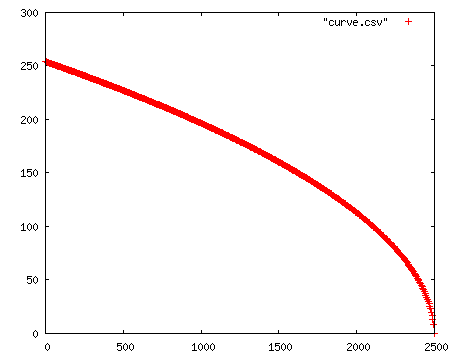
\includegraphics[width=\textwidth]{braking-curve}}
  \caption{Basic braking curve for EBD, target is at 2,500 m at speed
    0 km/h, deceleration is constant $-1 m/s^2$}
  \label{fig:braking-curve}
\end{figure}

After modeling several chapters of the SRS, we see following
advantages to using GNATprove:

\begin{itemize}
\item The model relies on the well known and well documented Ada
  language. It is easy to find documentation and tutorials on the web;
\item We were able to describe all the different kinds of entities
  found in the SRS: transition tables, algorithms, data structures,
  requirements on functional or data parts, etc. The description of
  data types is very expressive and thus helps writing a readable
  model. We are able to compute a basic braking curve (see figure
  \ref{fig:braking-curve}), which we consider a rather complex
  computation;
\item The description is rather concise, which we see as a very
  positive point;
\item By writing as comment the reference to the corresponding SRS
  paragraph, we have a basic but affective traceability. This approach
  could probably be automated, for example using tools to produce
  traceability matrix for verification purpose;
\item We were able to express formally most of requirements found in
  the SRS and prove part of those;
\item The model can be compiled and is executable. It can be
  interfaced with external entities like Graphical User Interface.
\end{itemize}

However some shortcomings have been identified:
\begin{itemize}
\item One needs to learn the Ada language in order to understand the
  model. The Ada language is big. The subset handled by GNATprove is
  nonetheless smaller and the concepts are quite well known for
  imperative languages (functions or procedures, variables, loops,
  records and arrays, ...);
\item The model is not graphical. Especially for model overview, a
  graphical understanding would be helpful. It might be possible to
  provide such a graphical overview using Ada tools;
\item One needs to build needed domain specific abstractions in order
  to write the model, e.g. the step functions defined in section
  \ref{sec:step-function}. But even if this effort is not negligible,
  once this is done it can be capitalized over several models or model
  parts;
\item The proofs are not complete and some parts cannot be done with
  the provided automated provers.
\end{itemize}

\section{A note on proofs}

One main goal of using GNATprove approach is to make proof on parts of
the model. We have attempted to make such proof:
\begin{itemize}
\item On exclusion property that should be fulfilled by transition
  table of SRS section 4.6. We can show that the exclusion cannot be
  proved without using external assumptions;
\item On the modeling of Step Functions. On them, we have proved most
  properties but some Verification Condition (VC) are not proved or
  cannot be proved.
\end{itemize}

Some formalization are generating a lot of VC, e.g. about 9,000 for
\Ada{Step_Function.Restrictive_Merge} function. This is going to be
fixed in the next release of GNATprove tool in
2013\footnote{\label{fn:gnatprove-improvements}\url{http://lists.forge.open-do.org/pipermail/hi-lite-discuss/2013-April/001270.html}}.

In case a VC is not proved, the GNATprove error message is sometimes
difficult to understand or even missing. This point is going to be
significantly improved in next release of GNATprove\footnote{Same
  reference as footnote \ref{fn:gnatprove-improvements}}.

GNATprove tool is handling quite well integer types. It is therefore
relatively easy to prove absence of Run Time Errors like overflow,
underflow or out-of-bound accesses. Regarding floating point numbers,
the situation is much less rosy. Even if a basic mapping to
Mathematical real numbers in the prover is provided, it is much more
difficult to prove range checks.

More fundamentally, we are formally specifying or verifying detailed
algorithms described in the SRS, but the underlying principles,
i.e. those related to safety, are not explicitely stated. Therefore we
are not sure such a modeling effort would be worth it for a real
development (except maybe for absence of Run Time Error).

\chapter{Detailed model description}

The model is organized into a set of ADS (Ada Package Specification)
or ADB (Ada Package Body or program) files. The ADS file declare each
function and procedure and optionally the contract it should fulfill
using \Ada{Pre =>} and \Ada{Post =>} notation. In those parts,
``\Ada{for all}'' stands for mathematical ``$\forall$'' and ``\Ada{for
  some}'' stands for ``$\exists$''. The ADB file contains code
corresponding to the function or procedure declaration. As we are
building a \emph{description} of the SRS without making it executable,
the ADB file is often empty or missing.

Each Ada package, an Ada ADS and an Ada ADB files, corresponds to a
section of the SUBSET-026 SRS. Each paragraph of the SRS is modeled by
one or more Ada data type definition or function definition. We have
extensively used user defined data type definition to strongly type
the different kinds of identifiers in the model. For example, an
\Ada{ertms_etcs_level_t} is a different integer that
\Ada{RBC_RIU_ID_t}.


\section{Generic parts of the model}

In this part, we define relatively simple data types or model
variables reused in other parts of the model.

\lstinputlisting[language=Ada,firstline=21]{../src/data_types.ads}
\lstinputlisting[language=Ada,firstline=21]{../src/etcs_level.ads}
\lstinputlisting[language=Ada,firstline=21]{../src/appendix_a_3_1.ads}


\subsection{SUBSET-026-4.3.2 ETCS modes}

\lstinputlisting[language=Ada,firstline=21]{../src/section_4_3_2.ads}


\section{SUBSET-026-4.6 Transitions between modes}

Here we define as Boolean variables each condition that should be
fulfilled or not to make a transition from one mode to another,
e.g. \Ada{driver_selects_shunting_mode}. In a more complete model,
those variables would probably be defined and handled in other
packages.

We then define a set of functions that correspond to each individual
condition defined in table §4.6.2 of the SRS. See for example
\Ada{condition_1}.

Those conditions are then in turn combined into a set of functions
defining the condition under which a mode transition can occur. See
for example \Ada{condition_transition_SB_to_SH}.

We end with a function \Ada{transition} of which \Ada{Contract_Cases}
expresses that the different transition condition should be disjoint
and complete, in order to prove it. This cannot be proved using only
the assumptions describe in §4.6 of the SRS. See
\url{https://github.com/openETCS/model-evaluation/wiki/Open-Question-for-Modeling-Benchmark#section-46}
for a detailed example. 

\lstinputlisting[language=Ada,firstline=21]{../src/section_4_6.ads}
\lstinputlisting[language=Ada,firstline=21]{../src/section_4_6.adb}


\section{SUBSET-026-3.5.3 Establishing a communication session}

In this section, we attempt to model SRS §3.5.3.

\subsection{Safe Radio package}

This package emulates an API to open a connection and send messages on
it.

\lstinputlisting[language=Ada,firstline=21]{../src/safe_radio.ads}
\lstinputlisting[language=Ada,firstline=21]{../src/safe_radio.adb}

\subsection{Com\_map utility package}

This package defines an abstract table that can be used to search if a
connection has already been established, is being established or is
not opened.

We have used an array for the definition of \Ada{Com_To_RBC_Map}. We
would have preferred to use Ada formal containers, but those cannot be
handled by GNATprove in its GPL 2012 edition.

\lstinputlisting[language=Ada,firstline=21]{../src/com_map.ads}

\subsection{Section 3.5.3 modeling}

The core of the model. We use the body of procedure
\Ada{Initiate_Communication_Session} to detail the algorithm specified
in the SRS.

\lstinputlisting[language=Ada,firstline=21]{../src/section_3_5_3.ads}
\lstinputlisting[language=Ada,firstline=21]{../src/section_3_5_3.adb}


\section{SUBSET-026-3.13 Speed and distance monitoring}

In this section we try to model the complex speed and distance
monitoring specified in SRS §3.13.

Contrary to previous parts of the model, some functions or procedures
have both a specification and a body thus they can be compiled and
executed as well as proved. We have done this work for
\Ada{Step_Function} and \Ada{Deceleration_Curve} packages.

\subsection{Generic package}

In this package we define some physic related data types (speed,
distance, deceleration, ...) and some utility functions (e.g. to
convert from m/s to km/h).

One should notice that in next release of GNAT GPL, it will be
possible to use a specific mechanism (\Ada{Dimension_System} aspect)
to describe those units, thus enabling more checks by the compiler.

\lstinputlisting[language=Ada,firstline=21]{../src/units.ads}
\lstinputlisting[language=Ada,firstline=21]{../src/units.adb}

\subsection{Modeling of step functions}
\label{sec:step-function}

In this package we model the step functions used throughout the
SRS. They are defined as an array of delimiters, to each delimiter
corresponding the value of the current step.

We define following functions:
\begin{itemize}
\item \Ada{Is_Valid}: returns \Ada{True} if the delimiters are in
  increasing order;
\item \Ada{Has_Same_Delimiters}: returns \Ada{True} if two step
  functions change their steps at the same positions;
\item \Ada{Get_Value}: returns the value of a step function at
  position \Ada{X};
\item \Ada{Minimum_Until_Point}: returns the minimum of a step
  function until a position \Ada{X};
\item \Ada{Restrictive_Merge}: merges two step functions into a third
  one, in such a way that the result is always the minimum of the two
  step functions.
\end{itemize}

All those functions can be compiled and tested (see examples below).

We have tried to prove them, but except for the simplest ones some
unproved and sometimes complex VCs are remaining.

\lstinputlisting[language=Ada,firstline=21]{../src/step_function.ads}
\lstinputlisting[language=Ada,firstline=21]{../src/step_function.adb}
\lstinputlisting[language=Ada]{../src/step_function_test.adb}

\subsection{Modeling of deceleration curves}

In this package, we have modeled deceleration curves and functions
computing them.

Function \Ada{Distance_To_Speed} is a simple function that returns the
distance to reach a final speed, given an initial speed and a constant
(and negative) acceleration. We have tried to prove this function.

Procedure \Ada{Curve_From_Target} computes the braking curve given as
input a target (speed and location). This computation is closer to SRS
SUBSET-026 requirements but albeit is not proved.

Procedure \Ada{Print_Curve} is a utility function to print the curve
on the terminal, in order to plot it.

\lstinputlisting[language=Ada,firstline=21]{../src/deceleration_curve.ads}
\lstinputlisting[language=Ada,firstline=21]{../src/deceleration_curve.adb}
\lstinputlisting[language=Ada]{../src/deceleration_curve_test.adb}

\subsection{Section 3.13.2 Train and Track-side related inputs}

This package is the model for all the input parameters used for
distance and speed monitoring algorithms.

Those functions can be compiled. No proof attempt has been made.

\lstinputlisting[language=Ada,firstline=21]{../src/sec_3_13_2_monitoring_inputs.ads}
\lstinputlisting[language=Ada,firstline=21]{../src/sec_3_13_2_monitoring_inputs.adb}

\subsection{Sections 3.13.4 to 3.13.8 Braking curves computation}

The following packages contains the modeling of the braking curves
computation, as close as possible to SRS §3.13.4 to §3.13.8.

\lstinputlisting[language=Ada,firstline=21]{../src/sec_3_13_4_gradient_accel_decel.ads}
\lstinputlisting[language=Ada,firstline=21]{../src/sec_3_13_6_deceleration.ads}
\lstinputlisting[language=Ada,firstline=21]{../src/sec_3_13_6_deceleration.adb}
\lstinputlisting[language=Ada,firstline=21]{../src/sec_3_13_8_targets_decel_curves.ads}
\lstinputlisting[language=Ada,firstline=21]{../src/sec_3_13_8_targets_decel_curves.adb}

%% \begin{figure}
%%   \centering
%%   \fbox{
\includegraphics[width=2in]{itea}}
%%   \caption{Yet Another Castle In Appendix}
%%   \label{fig:castle2}
%% \end{figure}

\bibliographystyle{abbrv}
\bibliography{GNATprove-model-report}


%===================================================
%Do NOT change anything below this line

\end{document}

% LocalWords:  GNATprove AdaCore's GPS VC pre adb GPL SMT Satisfiability ETCS
% LocalWords:  FIXME SRS VCs
